\documentclass[11pt]{article}
\usepackage{amsmath,amssymb,color,hyperref,graphicx,pdfsync}
\usepackage{textcomp}
\usepackage{setspace}
\usepackage{listings}
\usepackage{svn}
\SVN $Date$
\SVN $Revision$
\SVN $Author$
\SVN $HeadURL$
\newcommand\revisioninfo{\centerline{\textcolor{blue}{Revision: \SVNRevision ; Last changed by \SVNAuthor\ on \SVNDate .}}}

\graphicspath{{Figures/}}

\textwidth 5.5 truein
\oddsidemargin .5 truein
\evensidemargin .5 truein
\topmargin -.5 truein
\textheight 8.5in

\definecolor{gray}{gray}{0.5}
\definecolor{green}{rgb}{0,0.5,0}

\def\todo#1{\textcolor{blue}{{\bf To do:} #1}}
\def\question#1{\textcolor{red}{\bf Question:} #1}

%\def\code#1{{\ttfamily #1}}
\def\class#1{\textcolor{green}{\ttfamily\small #1}} % \bfseries
\def\fn#1{{\ttfamily\small #1}} % \ttfamily
\def\virtualfn#1{{\ttfamily\small\slshape #1}} % \itshape

\let\code\lstinline

\lstset{
language=C++,
basicstyle=\ttfamily\small\setstretch{1},
stringstyle=\color{blue},
showstringspaces=false,
keywordstyle=,
identifierstyle=,
columns=flexible,
commentstyle=\color{gray}\slshape,
emph={TimeStepper,ProjectionSolver,Motion}, % abstract base classes
emphstyle=\color{green}\slshape,
emph={[2]Euler,AdamsBashforth},
emphstyle={[2]\color{green}},
}

\begin{document}

\title{Design document for Immersed Boundary Projection Method (IBPM)}
\author{Clancy Rowley}
\date{\revisioninfo}
\maketitle

\section{Purpose of this document}
This document describes the design of a code to implement the fast (multiple-grid) Immersed Boundary Projection Method (IBPM) of Colonius and Taira \cite{ColTai-07}.  Here we give a high-level overview of the classes planned, interactions between them, and their public interfaces.  Where appropriate, we describe ideas for possible implementations, but for the most part we leave implementation to the detailed class design.

The design here addresses only the single-grid case, rather than the more complex multiple-grid case.  The philosophy here was that we will probably want to iterate and refine this design, and will learn along the way (for instance, when implementing the boundary conditions and learning more about the dependencies), so it probably does not make sense to design for multiple grids at the outset.

This document is not intended to be a ``living'' document that evolves as changes are made to the code, and thus should not be taken as the definitive documentation.  The intent is for the ``living'' documentation to be contained within the code itself, to be extracted using Doxygen, and for this document to serve both as a blueprint for construction, and as a reference for how and why design decisions were made.  If major changes to the structure are made, however (such as extending to the multiple-grid case), then it would be appropriate to revise this document, or write a new one.

\tableofcontents

\section{History and design approach}

\subsection{Previously used code and its limitations}
Prior to the development of the code described in this document, we have been using an implementation of the Immersed Boundary Projection Method (IBPM) written by Colonius and Taira, using Fortran 90.  However, because of the complexity and the tight coupling of the Fortran implementation, this code has become difficult to maintain.  For instance, we wished to change the timestepper, from a second-order Adams-Bashforth/Crank-Nicolson scheme (a two-step scheme) to a Runge-Kutta/Crank-Nicolson scheme, both for improved timestep restrictions, and to sidestep certain issues with a multi-step scheme, when used for adjoint simulations, eigenvalue solvers, and the like.  However, the Fortran~90 code is tightly coupled, making extensive use of global or global-like data (publicly accessible module data), and even making such a supposedly simple modification would require major surgery (in particular, to the long routine {\tt operators.f90::advance}, as well as {\tt myfft.f90::setup\_fft}).  Such modifications throughout the code would be error prone, and it would be difficult to switch between integrators, should one wish to go back to Adams-Bashforth, or try other timesteppers.  

Furthermore, the Fortran code has already become rather unwieldy, with flags for different modes of operation, such as solving the linearized or adjoint equations.  This implementation using flags has proven error-prone as well, since the switching logic is distributed throughout the code, and future modifications require a thorough knowledge of many parts of the code.

There are many other smaller reasons for revamping the design of this previous code, for instance improving the mechanism for reading input files, specifying geometries, and especially specifying the motion of moving bodies.  But another major reason for redesign is to facilitate testing, and in particular automated testing at the level of individual routines or groups of routines.  The extensive use of global-like data makes such automated testing difficult or impossible, further hampering the maintainability of the code as new features are added.

\subsection{Overview of design approach}
In order to overcome the difficulties described above, an object-oriented design approach is used here.  The reasons for this are as follows:
\begin{itemize}
	\item Using inheritance eliminates the need to have switching logic distributed throughout the code, for instance for different versions of timesteppers, or different equations of motion.  Furthermore, related operations such as nonlinear, linear, and adjoint versions of the equations of motion can inherit common portions from a parent class, avoiding the need to duplicate large sections of code, which creates more maintenance problems.
	\item Using classes to store private data needed only by certain portions of the code (such as evaluating terms in the Navier-Stokes equations) encapsulates these algorithms, and avoids the need for global-like data, leading to many advantages.  In particular, if one is simply using these routines, one can safely ignore their implementation, focusing only on the interfaces.
	\item Establishing clean, sensible interfaces allows one to test these routines much more easily, and in an automated fashion, which would greatly facilitate debugging, and ensure that new bugs are not introduced when new functionality is added.
\end{itemize}

A key point is to separate {\em interface} from {\em implementation}, so that code that provides a service (i.e., implements a particular algorithm) is cleanly separated (via the interface) from code that uses this service.  In this way, the implementation of various portions of the code can evolve without affecting the rest of the code, as long as the interface remains consistent.

\subsection{What the code does}
For details of the numerical method this code solves, see~\cite{ColTai-07}.  Here, we give only a brief overview.

\paragraph{Immersed boundary method}
The Navier Stokes equations are solved in two dimensions, using a streamfunction-vorticity formulation, and a finite-volume method.  Thus, fluxes are defined on cell edges, and scalars such as pressure and vorticity (circulation about one cell) are defined at cell centers.

Let $q$ denote the (vector-valued) velocity flux, $\psi$ the streamfunction, and $\gamma$ the circulation about a cell.  The no-slip boundary condition at the surface of an object are imposed by delta-function forces at the boundary locations, and $f$ is a vector of these force values.  The equations to be solved are given as (22) in~\cite{ColTai-07}:
\begin{align}
	\frac{d\gamma}{dt} + C^TE^T\tilde f &= \nu L\gamma + C^T(q\times\gamma),
		\qquad \gamma\big|_\partial = bc_\gamma
		\label{eq:navier_stokes}\\
	L\psi &= -\frac{1}{\delta^2}\gamma,\qquad \psi\big|_\partial = bc_\psi
		\label{eq:poisson}\\
	EC\psi &= u_B.
		\label{eq:no_slip}
\end{align}
The first equation is the momentum equation, the second is a Poisson equation for the streamfunction, and the third equation is a constraint representing the no-slip condition, so that velocities at the boundary points match prescribed velocities~$u_B$. The discrete operators in the above equation are described in the table below, where $\delta$ is the grid spacing and $\nu=1/Re$ is one over the Reynolds number.
\begin{center}
\begin{tabular}{ccp{3.7in}}
Operator & Maps & Definition\\
$C$ 	& $\psi\mapsto q$ & curl of a scalar\\
$C^T$ 	& $q\mapsto \gamma$ & curl of a vector in 2d\\
$S$ 	& $\gamma\mapsto\hat\gamma$ & discrete sin transform\\
$L=-C^TC$	& $\gamma\mapsto\gamma$ & Laplacian, analogous to $\triangle u = \nabla(\nabla\cdot u) - \nabla\times\nabla\times u$\\
$\Lambda$	& $\hat\gamma\mapsto\hat\gamma$ & eigenvalues of Laplacian\\
$E$ 	& $q\mapsto u_B$ & restriction of fluxes everywhere to velocities at boundary\\
$E^T$	& $f\mapsto q$ & regularization of forces at boundary points to fluxes everywhere\\
$D$		& $q\mapsto \varphi$ & divergence of a vector field
\end{tabular}
\end{center}
Here, $u_B$ is a vector of velocities at boundary points.  An important aspect of the method is that the curl operator~$C$ is chosen such that its range is in the nullspace of a discrete divergence operator~$D$, such that $DC=0$, and the continuity equation is satisfied for any streamfunction~$\psi$.  The discrete Laplacian $L$ is diagonalized by the discrete sin transform~$S$, and its eigenvalues are known analytically, so the Poisson equation~(\ref{eq:poisson}) can be solved efficiently.
To retrieve the fluxes $q$ from the streamfunction~$\psi$, we need to add in a (prescribed) potential flow solution~$q_\text{pot}$, so we have
\begin{equation}
	q = C\psi + q_\text{pot}.
\label{eq:compute_q}
\end{equation}
We consider farfield boundary conditions, for which $bc_\gamma$ in~(\ref{eq:navier_stokes}) and~$bc_\psi$ in~(\ref{eq:poisson}) are both zero.

\paragraph{Time discretization}
Equation~(\ref{eq:navier_stokes}--\ref{eq:no_slip}) are stepped forward in time using a projection method, as follows.  For instance, discretizing the linear terms of (\ref{eq:navier_stokes}) using Crank-Nicolson (trapezoidal rule), and the nonlinear terms using explicit Euler, one obtains
\begin{align}
	\left(1-\frac{\nu\Delta t}{2}L\right)\gamma^{n+1} + \Delta t C^TE^Tf &= \left(1 + \frac{\nu\Delta t}{2}L\right)\gamma^n + \Delta t C^T (q^n\times\gamma^n)  \label{eq:timestepper}\\
	-\frac{1}{\delta^2}ECL^{-1}\gamma^{n+1} &= u_B^{n+1}
\end{align}
These equations are of the form
\begin{equation}
	\begin{bmatrix}
		\mathcal{A} & \mathcal{B}\\\mathcal{C} & 0
	\end{bmatrix}
	\begin{bmatrix}
		\gamma^{n+1}\\ f
	\end{bmatrix}
	=
	\begin{bmatrix}
		a\\b
	\end{bmatrix}
\label{eq:constrained}
\end{equation}
where
\begin{align}
	\mathcal{A} &= 1 - \frac{\nu\Delta t}{2}L\\
	\mathcal{B} &= \Delta t C^TE^T\\
	\mathcal{C} &= -\frac{1}{\delta^2}ECL^{-1}\\
	a &= \left(1+\frac{\nu\Delta t}{2}L\right)\gamma^n + \Delta t C^T(q^n\times\gamma^n)\\
	b &= u_B.
\end{align}



\paragraph{Projection method}
We solve the constrained equation~(\ref{eq:constrained}) using the following algorithm:
\begin{equation}
\begin{aligned}
	\mathcal{A}\gamma^* &= a,\qquad \gamma^*\big|_\partial\\
	\mathcal{CA}^{-1}\mathcal{B}f &= \mathcal{C}\gamma^* - b\\
	\gamma^{n+1} &= \gamma^* - \mathcal{A}^{-1}\mathcal{B}f
\end{aligned}
\label{eq:projection_alg}
\end{equation}
Since the matrix $\mathcal{A}$ is easily invertible using a sin transform, one may solve the first equation easily (applying boundary conditions on~$\gamma^*$).  The second equation is rather small ($\text{\#forces} \times \text{\#forces}$), and furthermore the matrix $\mathcal{M}=\mathcal{C}\mathcal{A}^{-1}\mathcal{B}$ is symmetric, since $\mathcal{A}$ and $L$ have the same eigenvectors.  When the boundary conditions are fixed (stationary bodies), then the matrix~$\mathcal{M}$ is constant in time, and so may be LU decomposed (e.g. using a Cholesky decomposition) once beforehand, and solved rapidly at each timestep.  When the boundary conditions vary in time, then $E$ changes at each step, and a direct solve is not as efficient as an iterative solve, such as a conjugate-gradient method (also for symmetric matrices).

In the design below, we decouple the algorithm for the timestepper~(\ref{eq:timestepper}) from the algorithm (\ref{eq:projection_alg}) for solving equation~(\ref{eq:constrained}).

\subsection{Multi-domain method}
For large domains, it is not practical to use uniform grid spacing, so the method in~\cite{ColTai-07} uses a multi-domain approach in which several nested uniform grids are used.  The Poisson equations may still be solved efficiently in this case, also using a number of sin transforms, as outlined here.  We present a slightly modified version of this scheme that is slightly more accurate (the only real difference is in the definition of the operator $P^{k+1,k}$ that moves variables from a fine grid to a coarse grid).

One defines a scalar field $u$ on a nested set of grids $u^1,\ldots,u^{N_g}$, where $u^1$ is the finest grid and $u^{N_g}$ is the coarsest.  One then defines a sequence of {\em coarsening} operators $P^k$ that move points from the full grid to an individual coarse grid~$u^k$, by suitably averaging finer gridpoints.  These coarsening operators may be defined recursively, by starting with the finest grid and averaging values to each coarser grid sequentially.

In order to solve the system
\begin{equation}
	Lu = f,\qquad u\big|_\partial = bc_u,
\end{equation}
one first computes a sequence of coarsified forcing terms $f^1,\ldots,f^{N_g}$, for instance with $f^{k} = P^{k}f$. Then one considers the Laplacian $L_1$ on the finest (uniform) grid, and solves a sequence of Poisson problems
\begin{equation}
\begin{aligned}
	L_1 u^{N_g} &= 2^{N_g-1} f^{N_g},& u^{N_g}\big|_\partial &= bc_u\\
	L_1 u^{N_g-1} &= 2^{N_g-2} f^{N_g-1},& u^{N_g-1}\big|_\partial &= bc(u^{N_g})\\
	&\;\vdots\\
	L_1 u^1 &= f^1,& u^1\big|_\partial &= bc(u^2)
\end{aligned}
\end{equation}
where the operators $bc(u^{k+1})$ return the values on grid $u^{k+1}$ that are on the boundary of the next finer grid~$k$.  The scaling terms $2^k$ on the right-hand side compensate for the different grid spacings on the different domains.  Since the single-grid Laplacian $L_1$ is easily inverted using a sin transform, the overall solution is efficient.

One can show that with suitably defined coarsening operators, the process above {\em exactly} solves the original Poisson problem $Lu=f$, with the standard Laplacian operator on the full grid (second-order accurate in each sub-grid, first-order accurate at the boundaries).

\section{Classes}
In this section, we give a high-level description of the classes involved.  A diagram showing the main classes and their collaborations is shown in Figure~\ref{fig:class_diagram}.  Below, we discuss each of these and their interfaces in more detail.

\begin{figure}
\centering
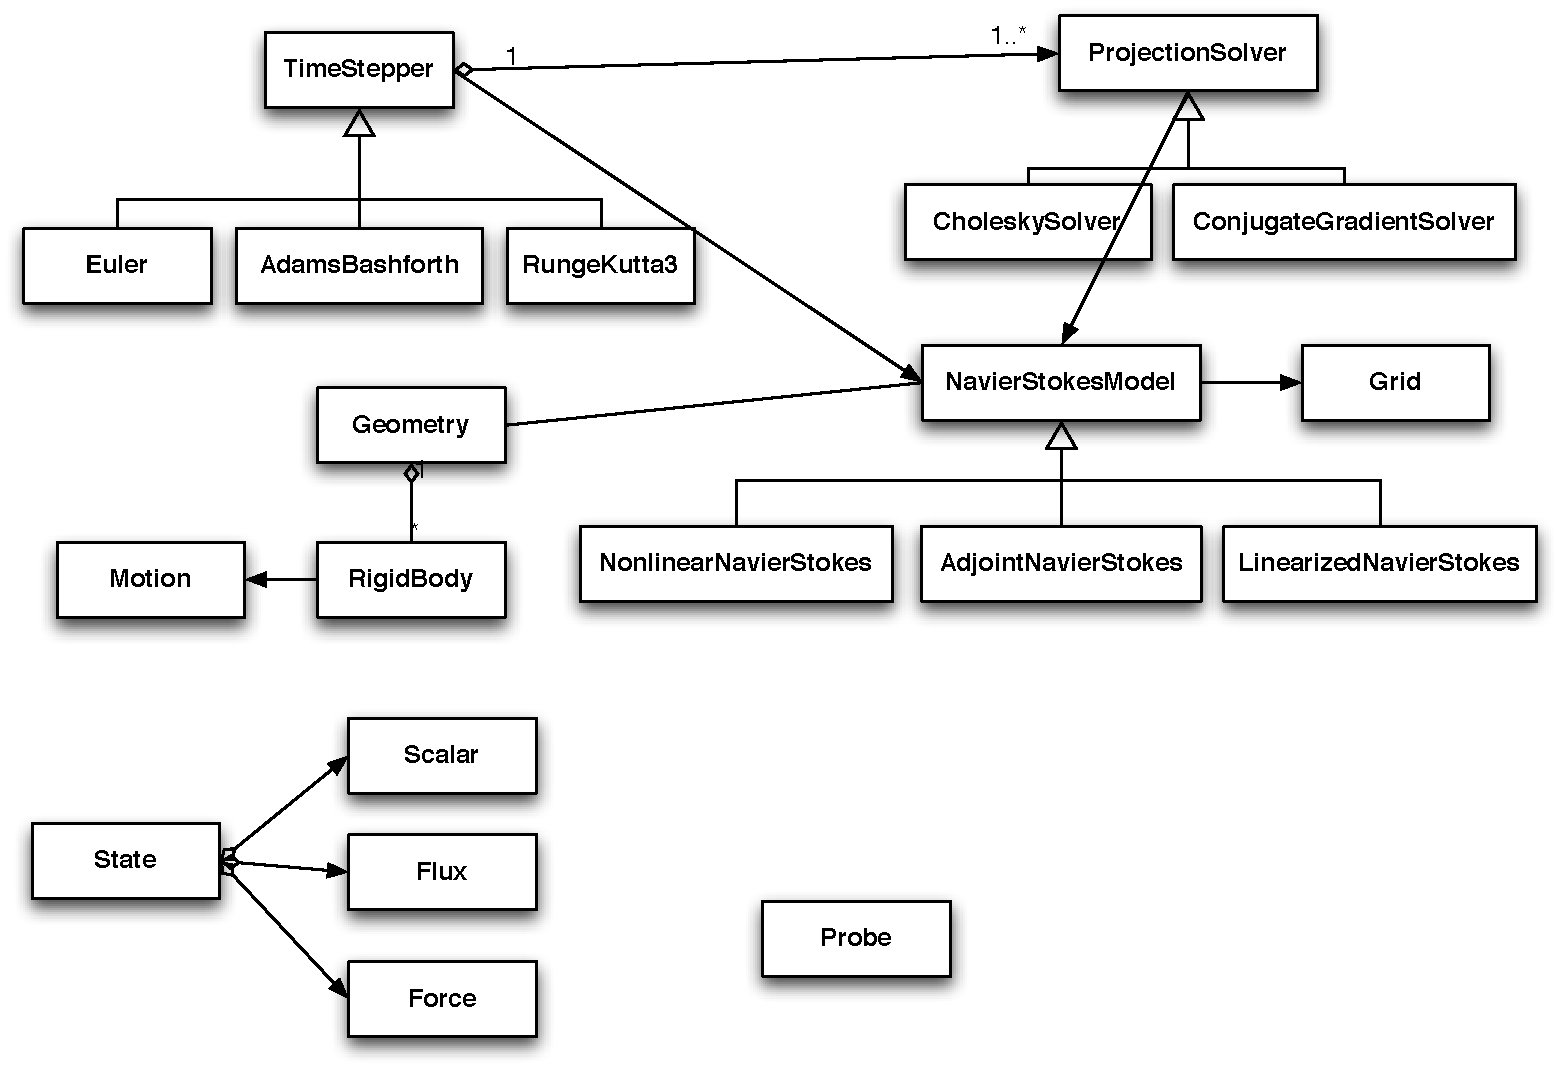
\includegraphics[width=0.95\linewidth]{IBFSDesign}
\caption{Diagram of classes and their collaborations.}
\label{fig:class_diagram}
\end{figure}

\subsection{TimeStepper}
Abstract base class to advance a flow field forward in time.

The governing equations are in the form
\begin{equation}
\begin{aligned}
\frac{d\gamma}{dt} + Bf &= L\gamma + N(q)\\
C\gamma &= b
\end{aligned}
\label{eq:model}
\end{equation}
where the operators in these equations are defined in the associated instance of \code|NavierStokesModel|.  Note that the nonlinear term depends only on the fluxes~$q$, but the fluxes can be computed from the circulation~$\gamma$ by~(\ref{eq:poisson},\ref{eq:compute_q}).

A \class{TimeStepper} instance (e.g. \class{AdamsBashforth}) has a method \fn{advance} that takes a \class{State}, and computes the value at the next timestep, overwriting the values passed in.  The instance has a pointer to a model (of type \class{NavierStokesModel}), which contains information about the \class{Grid} and \class{Geometry}, as well as the equations to be solved (e.g., \class{LinearNavierStokes}, \class{AdjointNavierStokes}), and instantiates its own \code|ProjectionSolver| as appropriate, for solving the projection step of the equations.  For instance, for a stationary body, the \class{CholeskySolver} should be used, and for moving bodies, for which the projection step in (\ref{eq:projection_alg}) varies at each timestep, an iterative solver such as the \class{ConjugateGradientSolver} is needed.

Note that \class{TimeStepper} is an abstract class, and cannot be instantiated directly.  One of its subclasses must be instantiated.

\paragraph{Interactions}
A \class{TimeStepper} object creates an appropriate \class{ProjectionSolver} object, which it uses for solving the projection step.  The terms $L$, $B$, $C$, and $N(x)$ are provided by a \class{NavierStokesSolver}.  The quantities to be stepped forward are contained in a \class{State}.

\paragraph{Interface}
\begin{description}
	\item \code|TimeStepper(NavierStokesModel& model, double timestep)|\\
		Constructor.  Setup all routines necessary to use \virtualfn{advance}, to step the solution forward by the given timestep.  Note that creation of the \class{ProjectionSolver} should be deferred to the subclasses, but determination of which type of solver to instantiate should be handled by the base class.
	\item \code|~TimeStepper()|\\
		Destructor.
	\item \code|virtual void advance(State& x) = 0|\\
	 	Advance the state $x$ forward one step, overwriting with the new value.  Pure virtual function: subclasses must override this.
\end{description}
\paragraph{Protected}
\begin{description}
	\item \code|ProjectionSolver* createSolver(double alpha)|\\
		Return a new \class{ProjectionSolver} of the appropriate type (e.g., conjugate gradient or Cholesky), with the appropriate initializations, e.g. for filename or tolerance.
	\end{description}

\paragraph{Design choices}
The \fn{createSolver} encapsulates the logic of choosing which solver to use, since this depends only on the \class{Geometry}, and in particular whether the body is stationary or moving.  This way, subclasses don't need to worry about this logic.  Note that some derived classes will need more than one solver.

\paragraph{Implementation}
The functionality of the projection step~(\ref{eq:projection_alg}) is contained in the \class{ProjectionSolver}, so the only portion derived classes need to implement when overriding \virtualfn{advance} is a description of the timestepper as in~(\ref{eq:timestepper}), followed by a call to \fn{\_solver.solve}(a,b,$\gamma^{n+1}$,$f^{n+1}$).  Note that a \class{CholeskySolver} should be instantiated when the body is stationary, while a \class{ConjugateGradientSolver} should be used when the body is moving, since the $B$ and $C$ matrices change at each step.

\subsubsection{Euler}
Timestepper using Crank-Nicolson for linear terms, Explicit Euler for nonlinear terms.

\paragraph{Interface}
\begin{description}
	\item \code|void advance(State& x)|\\
		Advance the state forward one step, overwriting with the new value.  
\end{description}

In particular, \fn{advance}$(\gamma,f)$ returns the solution of
	\begin{align}
		(1-\frac{h}{2}L)\gamma^{n+1} + hBf &= (1 + \frac{h}{2}L)\gamma^n + h N(q^n)\\
		C\gamma^{n+1} &= b_{n+1}
	\end{align}
where $h$ is the timestep.  Here, in the notation of~(\ref{eq:constrained}),
\begin{align}
	\mathcal{A} &= 1-\frac{h}{2} L\\
	\mathcal{B} &= hB\\
	\mathcal{C} &= C\\
	a &= (1+\frac{h}{2}L)\gamma^n + hN(q^n)\\
	b &= b_{n+1}
\end{align}
where quantities on the right-hand side are specified by the associated \class{NavierStokesModel}.

\subsubsection{AdamsBashforth}
Timestepper using Crank-Nicolson for linear terms, Adams Bashforth for nonlinear terms.

\paragraph{Interface}
\begin{description}
	\item \code|void advance(State& x)|\\
		Advance the state forward one step, overwriting with the new value.  If information about the previous timestep is available, use Adams-Bashforth for nonlinear terms; otherwise, use explicit Euler.
	\item \code|void setPreviousState(State& x)|\\
		Initialize the value of $x$ at the previous timestep.  Makes a copy of the necessary information internally.
\end{description}

In particular, \fn{advance}$(\gamma,f)$ returns the solution of
	\begin{align}
		(1-\frac{h}{2}L)\gamma^{n+1} + hBf &= (1 + \frac{h}{2}L)\gamma^n + \frac{h}{2} \big(3N(q^n) - N(q^{n-1})\big)\\
		C\gamma^{n+1} &= b_{n+1}
	\end{align}
where $h$ is the timestep.  Here, in the notation of~(\ref{eq:constrained}),
\begin{equation}
	a = (1+\frac{h}{2}L)\gamma^n + \frac{h}{2}(3N(q^n) - N(q^{n-1})
\end{equation}
with other parameters the same as \class{Euler}.

Note: storing the previous value~$N(q^{n-1})$ is the responsibility of \class{AdamsBashforth}.

\paragraph{Implementation}
Note that it is sufficient to store the nonlinear terms~$N(\gamma)$ at the previous timestep, rather than the whole state. This saves both memory and time, since the nonlinear terms need not be recomputed at the next step.

\subsubsection{RungeKutta2}
Timestepper using Crank-Nicolson for linear terms, RK2 for nonlinear terms.

Uses the scheme given by Peyret, p.~148\cite{Peyret:2002}, for $\alpha=1$, $\beta=1/2$:
\begin{align}
	(1 - \frac{h}{2}L)x_1 + hBf_1 &= (1+\frac{h}{2}L)x^n + hN(x^n)\\
	Cx_1 &= b_{n+1}\\
	(1-\frac{h}{2}L)x^{n+1} + hBf^{n+1} &= (1 + \frac{h}{2}L)x^n + \frac{h}{2}\big(N(x^n) + N(x_1)\big)\\
	Cx^{n+1} &= b_{n+1}
\end{align}
Note that the equations for $x_1$ correspond to an Euler-CN step.  Conveniently, both steps use the same values of $\mathcal{A}$, $\mathcal{B}$, and $\mathcal{C}$ as \class{Euler} and \class{AdamsBashforth}, so this scheme needs only one \class{ProjectionSolver}.

\paragraph{Interface}
\begin{description}
	\item \code|void advance(State& x)|\\
		Advance the state forward one step, overwriting with the new value.
\end{description}
		
\subsubsection{RungeKutta3}
Timestepper using Crank-Nicolson for linear terms, 3rd-order Runge-Kutta for nonlinear.

Uses the scheme given by Peyret, p.~149\cite{Peyret:2002}:
\begin{align}
	Q_1 &= hN(x^n)\\
	(1-\frac{h}{6}L)x_1 + \frac{h}{3}Bf_1 &= (1+\frac{h}{6}L)x^n + \frac{1}{3}Q_1\\
	Cx_1 &= b_{n+1/3}\\
	Q_2 &= -\frac{5}{9} Q_1 + hN(x_1)\\
	(1-\frac{5h}{24}L)x_2 + \frac{5h}{12}Bf_2 &= (1+\frac{5h}{24}L)x_1 + \frac{15}{16}Q_2\\
	Cx_2 &= b_{n+3/4}\\
	Q_3 &= -\frac{153}{128} Q_2 + hN(x_2)\\
	(1-\frac{h}{8}L)x^{n+1} + \frac{h}{4}Bf^{n+1} &= (1+\frac{h}{8}L)x_2 + \frac{8}{15}Q_3\\
	Cx^{n+1} &= b_{n+1}
\end{align}
In this case, we see that we have three different values for the matrices $\mathcal{A}$, $\mathcal{B}$ and $\mathcal{C}$, for the three different stages of the scheme, and three different calls to the \class{ProjectionSolver} are required.  Best to have three different instances of this solver, since in the stationary case, three different Cholesky factorizations need to be computed and stored.

\paragraph{Interface}
\begin{description}
	\item \code|void advance(State& x)|\\
		Advance the state forward one step, overwriting with the new value.
\end{description}
		
\subsection{ProjectionSolver}
Solve a system of the form
\begin{equation}
\begin{aligned}
	(1 - \frac{\alpha}{2}L)x + \alpha Bf &= a\\
	Cx &= b
\end{aligned}
\label{eq:projection_specific}
\end{equation}
for $f$ and $x$, using the algorithm~(\ref{eq:projection_alg}).  Note that this form of the equations arises for all of the timesteppers considered so far.  The parameter $\alpha$ is fixed, and the operators $L$, $B$, and $C$ are determined by an associated \class{NavierStokesModel}.

This is an abstract base class, and may not be instantiated directly.

\paragraph{Collaborations}
This class is used by \class{TimeStepper}, and contains a pointer to a \class{NavierStokesModel}.

\paragraph{Interface}
\begin{description}
	\item \code|ProjectionSolver(const NavierStokesModel& model, double alpha)|\\
		Constructor.  Setup all routines necessary to use \fn{solve}, including the protected methods \fn{Ainv}, \fn{B}, and \fn{C}.
	\item \code|~ProjectionSolver()|\\
		Destructor.
	\item \code|void solve(const Scalar& a, const BoundaryVector& b, Scalar& gamma, BoundaryVector& f)|\\
	 	Solve the system~(\ref{eq:projection_specific}) using the algorithm~(\ref{eq:projection_alg}.  Inputs are $a$ and $b$, and the solution is returned in $x$, $f$.
\end{description}
\paragraph{Protected methods}
\begin{description}
	\item \code|Scalar Ainv(const Scalar& x)|\\
		Compute $y = \mathcal{A}^{-1}x=(1+(\alpha/2)L)^{-1}x$ for a projection of the form~(\ref{eq:constrained})
	\item \code|Scalar B(const BoundaryVector& f)|\\
		Compute $y = \mathcal{B}f=\alpha Bf$, for a projection of the form~(\ref{eq:constrained}).
	\item \code|BoundaryVector C(const Scalar& x)|\\
		Compute $y = \mathcal{C}x=Cx$ for a projection of the form~(\ref{eq:constrained}).
	\item \code|BoundaryVector M(const BoundaryVector& f)|\\
		Compute $y = \mathcal{M}f=\mathcal{C}\mathcal{A}^{-1}\mathcal{B}f$, the matrix that must be inverted in the second step of the algorithm~(\ref{eq:projection_alg}).  Note that for the Navier-Stokes equations, this operator should be symmetric ($\mathcal{M}=\mathcal{M}^T$).
	\item \code|virtual BoundaryVector Minv(const BoundaryVector& b) = 0|\\
		Solve $\mathcal{M}f=b$ for $f$.  Pure virtual function: must be overloaded by subclasses.
	\item \code|Geometry* getGeometry()|\\
		Return a pointer to the associated \class{Geometry}.
\end{description}

\subsubsection{CholeskySolver}
Subclass of \class{ProjectionSolver}, in which $\mathcal{M}f=b$ is solved directly.

This class assumes the matrix~$\mathcal{M}$ is symmetric, and computes the Cholesky decomposition when it is instantiated.

\paragraph{Interface}
\begin{description}
	\item \code|CholeskySolver(const NavierStokesModel& model, double alpha)|\\
		Constructor.  Note that before using \fn{Minv} (needed by \fn{solve} in the base class), one must first call either \fn{computeCholesky} or \fn{loadCholesky}.
	\item \code|BoundaryVector Minv(const BoundaryVector& b)|\\
		Solve $\mathcal{M}f = b$ for $f$ directly using a Cholesky factorization already computed.
	\item \code|void computeCholesky()|\\
		Compute the Cholesky decomposition of~$\mathcal{M}$, storing it as private data.
	\item \code|bool loadCholesky(const string& fileName)|\\
		Load a Cholesky decomposition from the specified file.  Returns true if successful.
	\item \code|bool saveCholesky(const string& fileName)|\\
		Save a Cholesky decomposition to the specified file, overwriting if necessary.  Returns true if successful.
\end{description}

\paragraph{Design alternatives}
A different design would be for the constructor to take a filename as an argument (or deduce it from the name in the associated Geometry object), and automatically try to load the file, calling \fn{computeCholesky} if the file was not found, or was invalid.  However, the call to \fn{computeCholesky} can be time consuming, so it seems like a better design to have to explicitly call that, so the constructor does not mysteriously take a very long time.  The approach above also gives greater flexibility in using this class.

\paragraph{Implementation}
The factorization of $\mathcal{M}$ should of course be stored as private data.  One suggestion is to have a flag to check whether the factorization has been performed, and When saving and loading these factorizations, it would be good to save/load the name of the \class{Geometry} the configuration is being saved for.  This would allow a simple check whether a loaded file matches the current geometry.  Since the solver already knows about the geometry (through the \class{NavierStokesModel} instance passed to the constructor, made available through the \fn{getGeometry} method), this name does not need to be passed explicitly to the \class{CholeskySolver}.

\subsubsection{ConjugateGradientSolver}
Subclass of \class{ProjectionSolver}, in which $\mathcal{M}f=b$ is solved iteratively, using a conjugate gradient method.

This class assumes the matrix~$\mathcal{M}$ is symmetric, and iterates until a specified tolerance has been reached.

\paragraph{Interface}
\begin{description}
	\item \code|ConjugateGradientSolver(const NavierStokesModel& model, double alpha, double tolerance)|\\
		Constructor.  Store tolerance as private data.
	\item \code|void setTolerance(double tolerance)|
	\item \code|double getTolerance}()|
	\item \code|BoundaryVector Minv(const BoundaryVector& b)|\\
		Solve $\mathcal{M}f = b$ for $f$ iteratively, using a conjugate gradient method.
\end{description}


\subsection{NavierStokesModel}
Provide operators $L$, $B$, $C$, and $N(q)$ for a model of the form~(\ref{eq:model}).

The operators $B$, $C$, and~$N$ are specified directly, and $L$ is specified by transformations $S$ and $S^{-1}$ and a diagonal matrix $\Lambda$, such that $L=S^{-1}\Lambda S$.

This is an abstract base class, and may not be instantiated directly, but all operators are defined in the base class except for the nonlinear term~$N(q)$.  \todo{Look up how the nonlinear term should be computed, from refs in Tim's paper, or talking to Sunil.  Also look more carefully at the other operators to see whether they need boundary conditions passed as additional parameters, or what else should be included in the objects passed to them.}

\paragraph{Collaborations}
This class contains an instance of a \class{Grid} and \class{Geometry}, as well as a \class{Regularizer}, which contains operations to regularize values from the boundary to the grid, and interpolate from the grid to the boundary.

\paragraph{Interface}
\begin{description}
	\item \code|NavierStokesModel(const Grid& grid, const Geometry& geom, double Reynolds)|\\
		Constructor, given a specified \class{Grid} and \class{Geometry}, as well as the Reynolds number.  Set up the appropriate data needed to evaluate $\Lambda$, and the discrete sin transform $S$, $S^{-1}$.  Does not make a local copy of \class{Geometry}, but instead keeps a reference (or pointer) to the one passed.
	\item \code|~NavierStokesModel()|\\
	\item \code|Geometry* getGeometry()|\\
		Return a pointer to the associated \class{Geometry}.
	\item \code|Grid* getGrid()|\\
		Return a pointer to the associated \class{Grid}.
	\item \code|Scalar* getLambda()|\\
		Return a pointer to the eigenvalues $\Lambda$ of~$L$.
	\item \code|Scalar S(const Scalar& g)|\\
		Transform to eigenvectors of~$L$ (discrete sin transform).
	\item \code|Scalar Sinv(const Scalar& ghat)|\\
		Inverse transform $S^{-1}$.  Note that for the discrete sin transform, $S^{-1}$ should equal~$S$, but in some implementations, these may differ by a normalization constant.
	\item \code|Scalar B(const BoundaryVector& f)|\\
		Compute $\gamma = Bf$, as in~(\ref{eq:model}).
	\item \code|BoundaryVector C(const Scalar& gamma)|\\
		Compute $f = C\gamma$, as in~(\ref{eq:model}).
	\item \code|virtual Scalar nonlinear(const State& x) = 0|\\
		Compute nonlinear terms $y = N(x)$: pure virtual function, must be overridden by subclasses.
\end{description}

\paragraph{Protected}
\begin{description}
	\item \code|Scalar bilinear(const State& x1, const State& x2)|\\
		Return bilinear term, used by subclasses (e.g. $y = N(q)=\operatorname{bilinear}(q,q)$).
\end{description}

\paragraph{Design notes}
Note that some basic mathematical operations (such as curl of a vector, and of a scalar) are defined in the \class{Scalar} and \class{Flux} classes, so this class does not need to define such low-level operations.

Also note that the regularization operators ($E$ and $E^T$ in~(\ref{eq:model})) are not defined here.  Because these operations are also required in other parts of the code, unrelated to the Navier-Stokes solver (e.g. computing the lift and drag), it probably makes sense to encapsulate the regularization operators in a separate class, \class{Regularizer}.  The NavierStokesSolver could then point to an instance of Regularizer.

Another option is to define the \fn{regularize} operators in the \class{Geometry} class, so that they can be more easily updated when the body moves (then these updates occur only within one class).  However, this does not seem as appropriate, since otherwise \class{Geometry} does not need to know any information about the \class{Grid}, which is needed to compute regularization operators.


\subsubsection{NonlinearNavierStokes}
Define the nonlinear term for the full nonlinear Navier-Stokes equations.
\todo{Get the explicit form of this from Sunil, from Tim's papers, or from the old code.}
\paragraph{Interface}
\begin{description}
	\item \code|Scalar nonlinear(const State& x)|
\end{description}

\subsubsection{LinearNavierStokes}
Define the ``nonlinear'' term $N(q)$ for Navier-Stokes equations linearized about a base flow $x_0$.

\paragraph{Interface}
\begin{description}
	\item \code|LinearNavierStokes(const Grid& grid, const Geometry& geom, const State& baseflow)|\\
		Constructor for Navier-Stokes equations linearized about a constant equilibrium solution given by baseflow.
	\item \code|Scalar nonlinear(const State& x)|
\end{description}

\subsubsection{AdjointNavierStokes}
Define the ``nonlinear'' term $N(q)$ for adjoint Navier-Stokes equations, linearized about a base flow~$q_0$.  Note that, if the adjoint is defined with respect to an inner product weighted by the inverse Laplacian, then the adjoint equations differ from the linearized equations only in the nonlinear term, as described in~\cite{AhuRow-08}.

\paragraph{Interface}
\begin{description}
	\item \code|AdjointNavierStokes(const Grid& grid, const Geometry& geom, const State& baseflow)|\\
		Constructor for adjoint equations for Navier-Stokes linearized about a constant equilibrium solution given by baseflow.
	\item \code|Scalar nonlinear(const State& x)|
\end{description}

\subsection{Regularizer}
Define regularization operations that lift boundary vectors to a grid, and interpolate from a grid onto boundary locations.

Let $B$ denote a body, and $\xi\in\partial B$ denote points on the boundary.  Then, if $x\in\Omega$ denotes a point in the fluid domain~$\Omega$, we have, by definition of the delta function:
\begin{align}
	u(x) &= \int_\Omega u(\xi) \delta(x-\xi)\,d\xi\\
	u(\xi) &= \int_\Omega u(x) \delta(x-\xi)\,dx,
\end{align}
We discretize both of these integrals using a regularized version of the delta function, as in eq~(14) of~\cite{TaiCol-06}, and evaluate the integrals using quadrature.  In the discrete setting, the first equation is called {\em regularizing} from the boundary onto the grid, and the second is called {\em interpolating} from the grid onto the boundary.

\todo{What invariants should be satisfied by these, for testing?  For instance, what are the properties of the discrete delta function~(14) in~\cite{TaiCol-06}?  Should $\operatorname{Interpolate}\circ\operatorname{Regularize} = \operatorname{Identity}$?}

\paragraph{Interface}
\begin{description}
	\item \code|Regularizer(const Grid& grid, const Geometry& geom)|
	\item \code|void update()|\\
	Update operators, for instance when position of the bodies changes.
	\item \code|Flux toGrid(const BoundaryVector& u)|\\
	Regularize boundary data to grid
	\item \code|BoundaryVector toBoundary(const Flux& u)|\\
	Interpolate grid data to boundary
\end{description}

\paragraph{Collaborations}
Used by \class{NavierStokesModel} for including forcing terms and constraints, and by output routines that compute overall forces and moments on the bodies.

\paragraph{Implementation}
In order to compute the regularization, one needs to keep track of which cells are neighbors (within the region of support) of each boundary point.  More specifically, one needs to keep track of which horizontal/vertical forces or velocities are associated with each horizontal/vertical flux value, or vice versa.  In the Fortran 90 code, this is done as follows: for each flux index, one keeps track of a list of associated force indices, and a corresponding weighting factor for the association.  (Presumably, these weights need to satisfy an invariant, such as all weights for a given flux index or force index should sum to one, and this could be verified in tests.)

This is probably not the most efficient implementation, since many flux indices have no associated boundary points, and so these points do not need to be looped over in \fn{reg} or \fn{regT} in the Fortran code.  A better implementation is probably one of the following: for each boundary point, keep a list of associated flux points, and iterate over these; or just keep an unordered list of ``associations'' between flux indices and force indices, that can be looped over.  Note that it may be useful for other reasons to be able to look up the associated boundary points for each cell, but one never actually needs this for computing the regularization, or indeed anywhere else in the Fortran code.

\subsection{Grid}
Define parameters associated with an Eulerian grid.

A staggered grid is used, as shown in Figure~\ref{fig:grid}, with scalars (e.g., vorticity, streamfunction, pressure) defined at cell centers, and fluxes defined on cell edges.
\begin{figure}[htbp]
	\begin{center}
		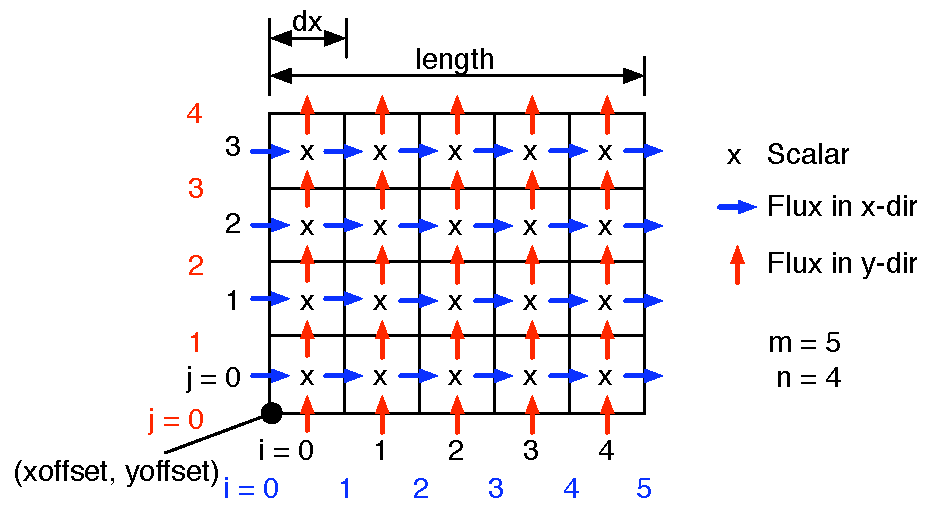
\includegraphics[width=4.5in]{Figures/grid.pdf}
	\end{center}
	\caption{Staggered grid of size $(m=5,n=4)$.}
	\label{fig:grid}
\end{figure}
We use single grid for now, but will want to extend to multiple grids.  (We choose to design the interface for a single grid first, so that we can iterate and refine the design before extending to multiple grids.)

\paragraph{Interface}
\begin{description}
	\item \code|Grid(int nx, int ny, double length, double xOffset, double yOffset)|\\
		Constructor, given numbers of gridpoints in $x$ and $y$-directions, length in the $x$-direction, and coordinates (\code|xOffset|, \code|yOffset|) of lower left gridpoint.  A square grid is assumed.
	\item \code|int getNx()|\\
		Return number of points in $x$-direction.
	\item \code|int getNy()|\\
		Return number of points in $y$-direction.
	\item \code|double getDx()|\\
		Return grid spacing (same in $x$- and $y$-directions).
	\item \code|double getXCenter(int i)|\\
		Return the $x$-coordinate of the center of cell $i$, in Fig.~\ref{fig:grid}, for $i\in[0,m-1]$.
	\item \code|double getYCenter(int j)|\\
		Return the $y$-coordinate of the center of cell $j$, in Fig.~\ref{fig:grid}, for $j\in[0,n-1]$.
	\item \code|double getXEdge(int i)|\\
		Return the $x$-coordinate of the left edge of cell $i$, in Fig.~\ref{fig:grid}, for $i\in[0,m]$.
	\item \code|double getYEdge(int j)|\\
		Return the $y$-coordinate of the bottom edge of cell $j$, in Fig.~\ref{fig:grid}, for $j\in[0,n]$.		
\end{description}


\subsection{State}
Include time, circulation about each cell (Scalar gamma), velocity flux in each direction (Flux q), and forces at the boundary (BoundaryVector f).

\paragraph{Interface}
\begin{description}
	\item \code|State(const Grid& grid, const Geometry& geom)|\\
		Constructor.  Allocate memory for the associated objects (flux, circulation, and forces).
	\item \code|~State()|\\
		Destructor.
\end{description}

\paragraph{Public data}
\begin{description}
	\item \code|int timestep|\\
		Timestep associated with the current value of the state (e.g. incremented by the \class{TimeStepper}).
	\item \code|double time|\\
		The time associated with the current value of the state (e.g. incremented by the \class{TimeStepper}).
	\item \code|Scalar gamma|\\
	\item \code|Flux q|\\
	\item \code|BoundaryVector f|
\end{description}

\paragraph{Implementation}
No need to store the Grid and Geometry information in the state, since it is already contained in the contained data structures.  This should probably be a \code|struct|, not a \code|class|, since it has only public data.

\subsection{Scalar}
Data structure and interface for storing a 2d array of scalars, located at cell centers (on multiple grids eventually).

\paragraph{Interface}
\begin{description}
	\item \code|Scalar(const Grid& grid)|\\
	Allocate memory for the 2d array.
	\item Access an element: \code|g(i,j)| for $i\in[0,m-1]$, $j\in[0,n-1]$.
	\item Addition/subtraction of two Scalars: \code|g1 + g2|
	\item Addition/subtraction of a double and a Scalar
	\item Multiplication of a Scalar by a double
	\item Retrieve x- and y-coordinates of the corresponding value:
	\begin{lstlisting}
x = omega.x(i,j);
y = omega.y(i,j);
x = omega.x(ind);
y = omega.y(ind);
	\end{lstlisting}
	\item Provide a type (\code|Scalar::index|) for accessing values.  For instance,
	\begin{lstlisting}
Scalar omega;
Scalar::index ind;
for (ind = omega.begin(); ind != omega.end(); ++ind) {
	omega(ind) = ...
}
ind = omega.getIndex(i,j)
	\end{lstlisting}
	\item \code|Scalar& curl(const Flux& q)|\\
	Set \code|*this| (the current Scalar) to the curl of q.  Returns \code|*this|.
	\item \code|Scalar& sinTransform(const Scalar& gamma)|\\
	Set \code|*this| to the discrete sin transform of the argument.  (Assumes different chunks of memory.)   Returns \code|*this|.
	\item \code|Scalar& sinTransformInv(const Scalar& gamma)|\\
	Set \code|*this| to the inverse discrete sin transform of the argument.   Returns \code|*this|.
	\item \code|Scalar& laplacian(const Scalar& gamma)|\\
	Set \code|*this| to the Laplacian of the argument.   Returns \code|*this|.
	\item \code|Scalar& laplacianInverse(const Scalar& gamma)|\\
	Assume zero boundary conditions for now (not for multiple grids).   Returns \code|*this|.
	\item \code|Scalar& divergence(const Flux& q)|\\
	Set \code|*this| to the divergence of the argument.   Returns \code|*this|.
	\item \code|double dot(const Scalar& g)|\\
	Return dot product of \code|*this| and argument.
	\item May need to provide direct access to the raw data in memory, for computing FFTs (experiment with FFTW to determine a good interface).
\end{description}

\paragraph{Implementation}
Laplacian and its inverse should probably be implemented using sin transform and multiplication by eigenvalues (as in f90 code).  Store this matrix of eigenvalues as private class data.

Probably implement using Blitz++, \code|Array<double,2>|.  Need to be able to take an FFT of this, so possibly want to allocate memory using an FFTW memory allocator (which ensures optimal alignment of doubles).  Governing principle: no matter what, make sure that the implementation of the arrays is independent from the interface, so the rest of the code does not need to change if the implementation is changed.

\subsection{Flux}
Data structure and interface for storing a 2D array of fluxes, located at cell edges.

\paragraph{Interface}
\begin{description}
	\item Addition/subtraction of Fluxes.
	\item Multiplication of Flux by a double.
	\item Access individual elements:
\begin{lstlisting}
Flux q(m,n);
q(X,i,j);   // i in [0,m]
            // j in [0,n-1]
q(Y,i,j);   // i in [0,m-1]
		    // j in [0,n]

\end{lstlisting}
	\item Retrieve x- and y-coordinates of the corresponding value:
	\begin{lstlisting}
x = q.x(dir,i,j);
y = q.y(dir,i,j);
x = q.x(ind);
y = q.y(ind);
	\end{lstlisting}
	\item Provide a type (\code|Flux::index|) for accessing values.  If two different Fluxes use the same grid, the same index can be used to access values from both Fluxes.  For instance,
	\begin{lstlisting}
Flux q1;
Flux q2;
Flux::index ind;
for (ind = q1.begin(); ind != q1.end(); ++ind) {
	q1(ind) = q2(ind) + ... // loop over all points
}
for (ind = q1.begin(X); ind != q1.end(X); ++ind) {
	// loop over fluxes in X-direction
}
for (ind = q1.begin(Y); ind != q1.end(Y); ++ind) {
	// loop over fluxes in Y-direction
}
ind = q.getIndex(dir,i,j)
	\end{lstlisting}
	
	\item \code|Flux& curl(const Scalar& f)|\\
	Set \code|*this| to the curl of the argument.  Returns \code|*this|.
	\item \code|Flux& gradient(const Scalar& f)|\\
	Set \code|*this| to the gradient of the argument.  Returns \code|*this|.
	\item \code|double dot(const Flux& q)|\\
	Return the dot product of \code|*this| and the argument.
	\item Provide an index type \code|Flux::Index| (and possibly an iterator) so that one can refer to individual elements and store these in array (for instance for implementing \code|regularize| in \class{NavierStokesModel}).
\end{description}

\subsection{BoundaryVector}
Data structure and interface for storing vectors located at boundary points (for instance, forces, velocities of the body, and positions of the boundary points).

\paragraph{Interface}
\begin{description}
	\item \code|BoundaryVector(int n)| \\
	Constructor, allocating memory for a body with $n$ points on the boundary.
	\item \code|BoundaryVector(int n, double* data)| \\
	Constructor using pre-existing data, as a 1d array (as returned by \fn{flatten} below).  Here $n$ is still number of boundary points, and \code|*data| has size~$2n$.
	\item \code|int getNumPoints()|\\
	Return the number of boundary points.
	\item \code|int getSize()| \\
	Return number of elements in the array, twice the number of points on the boundary.
	\item Addition/subtraction of BoundaryVectors of the same size.
	\item Multiplication of BoundaryVector by a double.
	\item \code|double *flatten()|\\
	Return a pointer to the data, expressed as a 1d C-style array.
	\item Access individual elements:
\begin{lstlisting}
f(X,i)		// i in [0,n-1]
f(Y,i)		// i in [0,n-1]
f(ind)
\end{lstlisting}
	\item Provide a type (\code|BoundaryVector::index|) for accessing values.  If two different BoundaryVectors have the same number of points, the same index can be used to access values from both BoundaryVectors.  For instance,
	\begin{lstlisting}
BoundaryVector f;
BoundaryVector f2;
BoundaryVector::index ind;
for (ind = f.begin(); ind != f.end(); ++ind) {
	f(ind) = f2(ind) + ... // loop over all points
}
for (ind = f.begin(X); ind != f.end(X); ++ind) {
	// loop over values in X-direction
}
for (ind = f.begin(Y); ind != f.end(Y); ++ind) {
	// loop over values in Y-direction
}
ind = f.getIndex(dir,i)
	\end{lstlisting}

	\item \code|double dot(const BoundaryVector& f)|\\
	Return the dot product of \code|*this| and the argument.
	
\end{description}

\paragraph{Routines}
\begin{description}
	\item \code|double InnerProduct(BoundaryVector& x, BoundaryVector& y)|
\end{description}

\paragraph{Design notes}
This class should be able to be used both for ``complete'' geometries (which may consist of multiple bodies), and for individual \class{RigidBody} objects.

The only operations needed to implement a conjugate gradient solver is vector addition, and scalar multiplication.  The \class{CholeskySolver} implementation, on the other hand, needs to access the elements stored in a 1d array, so should provide a method for returning a flattened version of 
In the Fortran code, this data was stored as a 1d array, to facilitate solving linear systems for forces.  Here we do not specify the implementation, and we should design this interface so that the solvers do not depend on this.

\subsection{Probe}
Store information about what information to write to probe files.

\todo{Flesh this out more.  Have a ProbeList or Logger class to collect different probes and call them when necessary?  Can postpone this until later.}

\subsection{Geometry}
Create, load, and save geometries composed of \class{RigidBody} objects.

This class is responsible for maintaining a list of bodies (each an instance of \class{RigidBody}, and for telling an associated \class{NavierStokesModel} when to update its regularization operators $E$ and $E^T$, for instance as used in~(\ref{eq:navier_stokes}).

Each geometry can be saved to or loaded from a file, and the interface should be designed so that it is easy to write a small utility program for creating and saving geometries (possibly with wrappers for Python or Matlab?).  

\paragraph{Interface}
\begin{description}
	\item \code|Geometry()| \\
		Constructor
	\item \code|~Geometry()| \\
		Destructor
	\item \code|void addBody(const RigidBody& body)| \\
		Append the given \class{RigidBody} to the list of bodies in the current geometry, making a copy of it internally.
	\item \code|void load(const istream& in)| \\
		Load a geometry from the specified input stream.  The format of the input file is as follows:
\begin{verbatim}
name My Geometry     # Comments indicated with '#'
body Flat plate
    line 0 0 1 0 50  # 50 points on a line
    center 0.25 0    # center at quarter chord
end
body Large Circle
    circle 2 3 5 100 # 100 points on a circle with radius 5, center (2,3)
                     # default center is (2,3)
end
body Airfoil
    raw naca0012.in  # Read in the raw data file
end
\end{verbatim}
	 Whitespace at the beginnings of lines is ignored, and comments are started by \#.
	\item \code|void setName(const string& name)| \\
		Set the name of the current geometry.
	\item \code|void setModel(const NavierStokesModel& model)| \\
		Set an associated \class{NavierStokesModel}.
	\item \code|void moveBodies(double time)| \\
		Update the position and velocities of the bodies, as specified by the associated \class{Motion}.  Also updates \fn{regularize} and \fn{regularizeT}, via the associated \class{NavierStokesModel}.
	\item \code|int getNumPoints()| \\
		Return the total number of points in all bodies.
	\item \code|BoundaryVector getPoints()| \\
		Return the list of coordinates for each point on each body.
	\item \code|BoundaryVector getVelocities()| \\
		Return the list of velocities at each point on each body.		
\end{description}

\paragraph{Design notes}
An alternative is to specify the operators \fn{regularize} and \fn{regularizeT} in this class, rather than \class{NavierStokesModel}.  See the remarks in \class{NavierStokesModel} for reasons why this interface was chosen.

\paragraph{Implementation}
Internally, either \class{Geometry} or each \class{RigidBody} should maintain a list of the points after the motion has been applied.  These will be necessary for defining the regularization operators, but don't need to be publicly accessible.  Not sure where is the best place to keep this information.

\subsection{RigidBody}
Specify coordinates and center of a rigid body, and its motion in time.

\paragraph{Interface}
\begin{description}
	\item \code|RigidBody()| \\
		Constructor.  Initialize the center to $(0,0)$.
	\item \code|void addPoint(double x, double y)| \\
		Add the specified point to the list of points on the body's boundary.
	\item \code|void addCircle(double xc, double yc, double radius, int numPoints)| \\
		Add a circle with center $(x_c,y_c)$ and the given radius, with the specified number of points.
	\item \code|void addLine(double x1, double y1, double x2, double y2, int numPoints)| \\
		Add a line connecting $(x_1,y_1)$ and $(x_2,y_2)$, with the specified number of points.
	\item \code|void load(istream& in)| \\
		Load a list of commands from the specified input stream.  See below for file format.
	\item \code|void loadRaw(istream& in)| \\
		Load a list of points, in ASCII format, with one point per line.  Assumes the center is 
	\item \code|void saveRaw(ostream& out)| \\
		Save a list of points to a file with the specified name, overwriting if already present.
	\item \code|int getNumPoints()| \\
		Return the number of points on the body's boundary.
	\item \code|BoundaryVector getPoints()| \\
		Return the list of coordinates for each point on the body.
	\item \code|bool isStationary()| \\
		Return true if the body is not moving in time.
	\item \code|void setMotion(Motion motion)| \\
		Set the evolution of the current body (which may be stationary or not).
	\item \code|void setCenter(double x, double y)| \\
		Set the center of the body, about which rotations are defined.
	\item \code|void getCenter(double& x, double& y)|\\
		Get the center of the body, about which rotations are defined.
	\item \code|void setName(string name)| \\
		Set the name of the body
	\item \code|string getName()| \\
		Return the name of the body
	\item 
\end{description}

\paragraph{File format}
Need to determine a good file format for loading/saving bodies.  ASCII is probably best, in some format easily readable by both humans and machines.  Example file format:
\begin{verbatim}
name some object
center x y
point x y
point x y
point x y
line x1 y1 x2 y2 npts
circle xc yc radius npts
raw naca0012.dat
end
\end{verbatim}
Commands should be read until the end of file is reached, or until {\tt end} is read (so that a single Geometry file can contain multiple bodies).

These commands easily map to the methods in the \class{RigidBody} interface, and are much more readable by humans than a raw list of points.  Could easily write a utility for parsing this and converting to a list of points for plotting with Matlab, Tecplot, etc.  Note that this format contains more information than a list of points, since it says something about the structure/connectivity.

\paragraph{Implementation}
Note that if saving to a file, need to save the information in the RigidBody with more structure, e.g. specifying Point, Line, Circle objects.  Probably best to implement more simply first, just as a raw list of points, and then make more complex if needed.

\subsection{Motion}
Specify a position and orientation as a function of time.

Abstract base class, must be subclassed to be instantiated.

\paragraph{Interface}
\begin{description}
	\item \code|Motion()| \\
		Constructor.
	\item \code|virtual bool isStationary()| \\
		Return false.  (Can be overridden by subclasses.)
	\item \code|virtual TangentSE2 getTransformation(double time) = 0| \\
		Return a Euclidean transformation and its velocity (an element of $TSE(2)$) at the specified time.
\end{description}

\paragraph{Design notes}
\fn{isStationary} returns False by default, since presumably the only subclass that would return true is \class{FixedPosition}.  Would probably be better style to make this a pure virtual function, but this way saves a little effort when making subclasses.

\subsubsection{FixedPosition}
Subclass of \class{Motion}, for a stationary body.

\paragraph{Interface}
\begin{description}
	\item \code|FixedPosition(double x, double y, double theta)| \\
		Define a \class{Motion} corresponding to a fixed position, rotation about the center.
	\item \code|bool isStationary()|\\
		Return true.
	\item \code|TangentSE2 getTransformation(double time)|\\
		Returns fixed transformation for all time: \code|TangentSE2(x,y,theta,0,0,0)|.
\end{description}


\subsection{SE2}
An abstraction of the group $SE(2)$ of translations and rotations in 2D.

Store these transformations $(x,y,\theta)\in SE(2)$, and provide their actions on points in $\mathbb{R}^2$.

\paragraph{Interface}
\begin{description}
	\item \code|SE2(double x, double y, double theta)|\\
		Constructor for a transformation corresponding to rotation by $\theta$, followed by translation by $(x,y)$.
	\item \code|void map(double a, double b, double& a_new, double& b_new)|\\
		Given the point~$(a,b)$, compute the mapped point~$(a_\text{new},a_\text{new})$.
\end{description}

Note: probably do not actually need this class in the main code, unless \code|TangentSE2| wants to use this class.

\subsection{TangentSE2}
An abstraction of the group $TSE(2)$ of translations and rotations in 2D, and their velocities.

Store the base point $g=(x,y,\theta)\in SE(2)$, as well as the tangent vector $\dot g=(\dot x, \dot y, \dot\theta)\in T_g SE(2)$.  Provide their actions $\Phi$ on points $(a,b,0,0)\in\mathbb{R}^2\times\mathbb{R}^2$:
\[\Phi_g \cdot (a,b,0,0) = (a_\text{new},b_\text{new},u_\text{new},v_\text{new})\]
where here the first two components $(a,b)$ are treated as ``points'' in the plane, and the second two components $(u,v)$ are treated as ``velocities'' in the plane.  Note that here we need only consider the case where the original (reference) velocity is zero, since the bodies are rigid, so the ``reference'' positions of the points on the boundary are fixed.

\paragraph{Interface}
\begin{description}
	\item \code|TangentSE2(double x, double y, double theta, double xdot, double ydot, double thetadot)|\\
		Constructor where the base point is $g=(x,y,\theta)\in SE(2)$, and the tangent vector is $\dot g=(\dot x, \dot y, \dot\theta)\in T_g SE(2)$.
	\item \code|void setPosition(double x, double y, double theta)|
	\item \code|void getPosition(double& x, double& y, double& theta)|
	\item \code|void setVelocity(double xdot, double ydot, double thetadot)|
	\item \code|void getVelocity(double& xdot, double& ydot, double& thetadot)|
	\item \code|void mapPosition(double a, double b, double& a_new, double& b_new)|\\
		Given the point $(a,b)$, compute the mapped point $(a_\text{new},b_\text{new})$.
	\item \code|void mapVelocity(double a, double b, double& u_new, double& v_new)|\\
		Given the point $(a,b)$ (with zero initial velocity), compute the mapped velocity $(u_\text{new},v_\text{new})$.
 \end{description}



\bibliographystyle{abbrv}
\bibliography{jabbrv,master}

% \begin{thebibliography}{1}
% 
% \bibitem{ColTai-07}
% T.~Colonius and K.~Taira.
% \newblock A fast immersed boundary method using a nullspace approach and
%   multi-domain far-field boundary conditions.
% \newblock {\em Comp.\ Meth.\ Appl.\ Mech.\ Eng.}, 197(25-28):2131--46, 2008.
% 
% \end{thebibliography}

\end{document}
